\documentclass[12pt]{article}
\usepackage{geometry}
\geometry{a4paper}


\usepackage{color}
\usepackage{hyperref}
\usepackage{amsmath}
\usepackage{amsfonts}
\usepackage{amssymb}
\usepackage{graphicx}
\usepackage{tcolorbox}
\usepackage{listings}
\usepackage{here}
\usepackage{txfonts}
\usepackage{algorithm}
\usepackage{algorithmic}
\usepackage{siunitx}
\usepackage{xcolor}
\usepackage{ascmac}
%\usepackage{fancybx}

\lstset {language = c++,
  basicstyle = \ttfamily \scriptsize,
  commentstyle = \textit,
  frame = tRBl,
  framesep = 5pt,
  showstringspaces = false,
  numbers = left,
  stepnumber = 1,
  numberstyle = \tiny,
  tabsize = 2,
  keywordstyle = \bfseries \color{blue},
  stringstyle=\color{magenta},
  commentstyle=\color{red},
  morecomment=[l][\color{red}]{\#}
  showstringspaces=false, % don't mark spaces in strings
}
\newcommand{\bi}[1]{\mathbf{#1}}
\newcommand{\bs}[1]{\boldsymbol{#1}}  % bold for greek characters
\newcommand{\bbR}{\mathbb{R}}

\author{Nobuyuki Umetani}

\title{Parameterization of the 3D Rotation \footnote{I 'm writing this note to keep in mind what I learned when I was MSc student}}

\begin{document}
\maketitle
\tableofcontents


\section{Introduction}

% Formulate the three-dimensional rigid body motion. Numerous mass points continuously displace each elastic body, discretization is necessary to express the displacement field in the computer, but because the distortion does not occur in the rigid body internally, the degree of freedom is the translation and the rotation It is possible to describe the state completely with only six degrees of freedom.
% First we will explain the axial vector. The rotation matrix can be written using this axial vector. We also explain rotation parameters that briefly describe the rotation matrix. By using the axial vector and rotation matrix, it is possible to formulate the rotation matrix and the variation of angular velocity. We derive the equation of motion by using the Hamiltonian principle. Finally, the incremental calculation of the equation of motion will be explained. \\

\section{Notation and Vector Calculus}

For arbitrary three dimensional vector $\bi{a}$, We denote skew-symmetric matrix (antisymmetric matrix) $\tilde{\bi{a}}\in\mathbb{R}^{3\times 3}$ such as
%
\begin{eqnarray}
\tilde{\bi{a}}=\left[\begin{array}{lll}0 & -a_3 & a_2 \\ a_3 & 0 & -a_1 \\ -a_2 & a_1 & 0 \end{array}\right]
\end{eqnarray}
%
The matrix-vector product with this matrix is equivalent to the exterior product (cross product)
%
\begin{equation}
\bi{a}\times\bi{b} = \tilde{\bi{a}}\bi{b}.
\end{equation}
%
The component of this skew-symmetric matrix can be written as:
%\textbf{}
\begin{equation}
\tilde{\bi{a}} = -\epsilon_{ijk}a_k \bi{e}_i\otimes\bi{e}_j,
\end{equation}
%
where $\epsilon$ is the \emph{Levi-Civita symbol}.

As follows, if we change the order of this skew-symmetric matrix and vector, the sign is changed.
%
\begin{eqnarray}
\tilde{\bi{a}}\bi{b}
&=&
\left\{\begin{array}{l}
-a_3b_2+a_2b_3\\
+a_3b_1-a_1b_3\\
-a_2b_1+a_1b_2
\end{array}\right\} \\
&=&
-\left\{\begin{array}{l}
-b_3a_2+b_2a_3\\
+b_3a_1-b_1a_3\\
-b_2a_1+b_1a_2
\end{array}\right\}\\
&=&
-\tilde{\bi{b}}\bi{a}\\
\Leftrightarrow \tilde{\bi{a}}\bi{b} &=& -\tilde{\bi{b}}\bi{a}
\end{eqnarray}\\

We multiply a vector to the left hand side of a skew-matrix to get this:
%
\begin{equation}
\bi{a}^T\tilde{\bi{b}} = -\bi{b}^T\tilde{\bi{a}}
\end{equation}

The product of two skew-matrices can be written as;
\begin{eqnarray}
\tilde{\bi{a}}\tilde{\bi{b}}
&=&
\left[\begin{array}{lll}
0 & -a_3 & a_2 \\
a_3 & 0 & -a_1 \\
-a_2 & a_1 & 0
\end{array}\right]
\left[\begin{array}{lll}
0 & -b_3 & b_2 \\
b_3 & 0 & -b_1 \\
-b_2 & b_1 & 0
\end{array}\right]\\
&=&
\left[\begin{array}{ccc}
-a_2b_2-a_3b_3 & a_2b_1 & a_3b_1 \\
a_1b_2 & -a_1b_1-a_3b_3 & a_3b_2 \\
a_1b_3 & a_2b_3 & -a_1b_1-a_2b_2
\end{array}\right]\\
&=&
\left[\begin{array}{ccc}
a_1b_1 & a_2b_1 & a_3b_1 \\
a_1b_2 & a_2b_2 & a_3b_2 \\
a_1b_3 & a_2b_3 & a_3b_3
\end{array}\right]
-(a_1b_1+a_2b_2+a_3b_3)\left[\begin{array}{lll}
1 & 0 & 0\\
0 & 1 & 0 \\
0 & 0 & 1
\end{array}\right]\\
&=& \bi{b}\bi{a}^T-(\bi{a}^T\bi{b})I
\end{eqnarray}

% Using this, let's calculate a matrix with a tilde once again for a vector with a tilde vector added to the vector.
Using the expression below we can do following transformation:
%
\begin{eqnarray}
\widetilde{\tilde{\bi{a}}\bi{b}}
&=&
\left[\begin{array}{lll}
0 & a_2b_1-a_1b_2 & +a_3b_1-a_1b_3 \\
-a_2b_1+a_1b_2 & 0 & +a_3b_2-a_2b_3 \\
-a_3b_1+a_1b_3 & -a_3b_2+a_2b_3 & 0
\end{array}\right]\\
&=&
\left[\begin{array}{lll}
a_1b_1 & a_2b_1 & a_3b_1 \\
a_1b_2 & a_2b_2 & a_3b_2 \\
a_1b_3 & a_2b_3 & a_3b_3
\end{array}\right]
-  \left[\begin{array}{lll}
a_1b_1 & a_1b_2 & a_1b_3 \\
a_2b_1 & a_2b_2 & a_2b_3 \\
a_3b_1 & a_3b_2 & a_3b_3
\end{array}\right]\\
&=& \bi{b}\bi{a}^T - \bi{a}\bi{b}^T = 2 asym(\bi{b}^T\bi{a})\\
&=& \{\bi{b}\bi{a}^T-(\bi{a}^T\bi{b})I\} - \{\bi{a}\bi{b}^T-(\bi{b}^T\bi{a})I\}\\
&=& \tilde{\bi{a}}\tilde{\bi{b}} - \tilde{\bi{b}}\tilde{\bi{a}}
\end{eqnarray}

%this is
Using the notation of cross product $\times$, this can be written as:
%
\begin{eqnarray}
(\bi{a} \times \bi{b}) \times \bi{v}
&=& - \bi{v} \times (\bi{a} \times \bi{b})\\
&=& \bi{v} \times ( \bi{b}\times \bi{a})\\
&=& \bi{b}(\bi{v} \cdot \bi{a} )-(\bi{v}\cdot \bi{b})\bi{a}\\
&=& \{ \bi{b}\bi{a}^T- \bi{a}\bi{b}^T\} \bi{v}
\end{eqnarray}

Corresponds to that holds. Let's calculate the process of applying the same outer product multiple times using this relationship.

\begin{eqnarray}
\bi{a}\times (\bi{a}\times (\bi{a}\times \bi{v}))
&=& \bi{a}\times\{\bi{a}(\bi{a}\cdot \bi{v})-(\bi{a}\cdot \bi{a})\bi{v}\}\\
&=& (\bi{a}\times \bi{a})(\bi{a}\cdot \bi{a})-(\bi{a}\cdot \bi{a})(\bi{a}\times \bi{v})\\
&=& -|a|^2(\bi{a}\times \bi{v})
\end{eqnarray}

. If you apply the same outer product $\tilde{\bi{a}}$ twice, you can see that only $-|a|^2$ is scalar multiplied. Therefore,

\begin{equation}
\tilde{\bi{a}}^3=\tilde{\bi{a}}\tilde{\bi{a}}\tilde{\bi{a}}=-|a|^2\tilde{\bi{a}}
\end{equation}


\begin{equation}
\tilde{\bi{a}}^4=-|a|^2\tilde{\bi{a}}^2
\end{equation}
%. Repeatedly using this,
We apply this transformation recursively to obtain
%
\begin{eqnarray}
\left\{\begin{array}{lll}\tilde{\bi{a}}^{2n-1}&=&(-1)^{n-1}|a|^{2(n-1)}\tilde{\bi{a}}\\ \tilde{\bi{a}}^{2n}&=&(-1)^{n-1}|a|^{2(n-1)}\tilde{\bi{a}}^2\end{array}\right.
\end{eqnarray}
% Holds.
\ \ \ \


For an orthogonal matrix (ie rotation) whose determinant is 1 $\bi{R}$,

\begin{equation}
(\bi{R}\bi{e}_1)\times (\bi{R}\bi{e}_2) = \bi{R}(\bi{e}_1\times\bi{e}_2) = \bi{R}\bi{e}_3
\end{equation}
%
Using this relationship, we have
%
\begin{equation}
\widetilde{\bi{R}\bi{v}} = \bi{R}\tilde{v}\bi{R}^T
\end{equation}



This is not limited to conversion by a general orthogonal matrix $V\;(V^{-1} =V^T )$.

For the transformation ($\det V = -1$) including mirror image transformation, it is understood that the sign is reversed as follows.

\begin{equation}
\widetilde{Vu} = -V\tilde{u}V^T
\end{equation}
A vector with such property is called \emph{pseudo vector}.



%%%%%%%%%%%%%%%%%%%%%%%%%%%%%%%%%%%%
%%%%%%%%%%%%%%%%%%%%%%%%%%%%%%%%%%%%
\section{Parameterization of Rotation}

Three dimensional rotation specifies linear transformation from a three dimensional vector to a three dimensional vector.
%
Therefore, it can be written as a 3x3 matrix.
%
However, due to the orthogonality constraints, these nine components of the matrix can not take arbitrary value independent.
%
We can, the rotation can be represented using three or four parameters.
% Three-dimensional rotation is expressed as a 3 × 3 matrix because it is a linear transformation from three-dimensional vector to three-dimensional vector, but due to the restriction that it has orthogonality, nine components of the matrix should take independent values ​​arbitrarily And can be represented by a smaller number of parameters.
% In general it can be expressed using 3 or 4 parameters. \\

Parameterization of rotation is important not only for reducing variables but also for interpolation. If you want to find a rotation and an intermediate rotation between a rotation, you can not average the rotation matrix. The average of the components of the two rotation matrices is no longer a rotation matrix. However, since the parameter can always be converted to a rotation matrix, it is possible to average the parameters and obtain an intermediate rotation matrix therefrom. \\

Typical parameters are given below.

\begin{itemize}
\item Euler angle
\item Bryant angle
\item Cartesian rotation vector
\item Rodrigues parameter
\item Euler parameter (Quaternion)
\item Conformal Rotation Vector (CRV)
\end{itemize}

Euler Angle and Bryant Angle take a parameterization method of how much an object is rotated along the regular coordinate axes on the object and three coordinate axes on the space, whereas Cartesian rotation vector, Rodrigues parameter and Euler parameter And Conformal rotation vector parameterize the object by rotating it around a certain vector. The former is easy to understand intuitively, but since there are problems such as gimbal lock, in general the latter parameters are used inside the calculation. \\

Each parameter will be described below.


%%%%%%%%%%%%%%%%%%%%%%%%%%%%%%%%%%%%
\subsection{Cartesian Rotation Vector}

Suppose the following vector $\bi{\Psi}$ represents a rotation rotated by $\theta$ around the unit vector $\bi{n}$.

\begin{equation}
\bi{\Psi} = \bi{n}\theta
\end{equation}

The rotation matrix can be written as follows.

\begin{tcolorbox}[title=rotation matrix]
\begin{equation}
\bi{R} = \bi{I} + \sin\theta\tilde{\bi{n}} + (1-\cos\theta)\tilde{\bi{n}}\tilde{\bi{n}}
\end{equation}
\end{tcolorbox}


\begin{figure}
\begin{center}
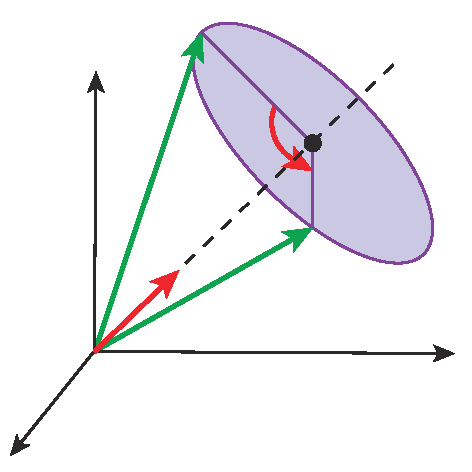
\includegraphics[width=80mm]{images/CartesianRotation.pdf}
\caption{Vector rotation with Cartesian Rotation Vector}
\end{center}
\end{figure}

\subsubsection{Infinitesimal Rotation Approximation}

At $|\Psi|=\theta<<1$ it is Infinitesimal rotation. Since $\sin(\theta)\simeq\theta,(1-\cos(\theta))\simeq\theta^2/2$ holds at this time, the rotation matrix can be approximated as follows.


\begin{eqnarray}
\bi{R} \simeq \bi{I} + \theta\tilde{\bi{n}} + \frac{\theta^2}{2}\tilde{\bi{n}}\tilde{\bi{n}}
&=& \bi{I} + \tilde{\bi{\Psi}} + \frac{1}{2}\tilde{\bi{\Psi}}\tilde{\bi{\Psi}}\\
&=&  \bi{I} + \tilde{\bi{\Psi}} - \frac{1}{2}|\Psi|^2\bi{I}\\
&=& \left(1- \frac{1}{2}|\Psi|^2\right)\bi{I} + \tilde{\bi{\Psi}}
\end{eqnarray}

This approximation is second-order accuracy, but if we consider $(1-\cos(\theta))\simeq0$ simply considering first-order accuracy, we can approximate as follows.

\begin{tcolorbox}[title=infinitesimal rotation (1st order approximation)]
\begin{equation}
\bi{R} \simeq \bi{I} + \theta\tilde{\bi{n}} = \bi{I} + \tilde{\bi{\Psi}}
\end{equation}
\end{tcolorbox}



\subsubsection{Rodrigue's rotation formula}

Using $\tilde{\bi{a}}\tilde{\bi{b}} = \bi{a}\bi{b}^T - (\bi{a}^T\bi{b})\bi{I}$ for this expression, the rotation matrix can be transformed as follows.

\begin{eqnarray}
\bi{R}
&=& \bi{I} + \sin\theta\tilde{\bi{n}} + (1-\cos\theta)(\bi{n}\bi{n}^T-||\bi{n}||^2\bi{I})\\
&=& \cos\theta\bi{I} + \sin\theta\tilde{\bi{n}} + (1-\cos\theta)\bi{n}\bi{n}^T
\end{eqnarray}

This formula is called Rodrigue's rotation formula.

\begin{tcolorbox}[title=Rodrigue's rotation formula]
\begin{equation}
\bi{R} = \cos\theta\bi{I} + \sin\theta\tilde{\bi{n}} + (1-\cos\theta)\bi{n}\bi{n}^T
\end{equation}
\end{tcolorbox}


\subsubsection{Rotation Matrix as a Exponential Function}

The rotation matrix can also be interpreted by infinitely small sets of small rotations as follows. This can be written from the definition of the operator on the shoulder of the index as follows.

\begin{equation}
\bi{R}(\bi{\Psi}) = \lim_{n\rightarrow\infty}\left\{1+\frac{1}{n}\tilde{\bi{\Psi}}\right\}^n =exp{\tilde{\bi{\Psi}}}
\end{equation}

Now, if we transform the equation as follows, it turns out that the definition of rotation using this exponential function gives the same rotation matrix. However, in this case, the relational expression of $\tilde{\bi{\Psi}}\tilde{\bi{\Psi}}=-|\Psi|^2\bi{I}$ is used.

\begin{eqnarray}
\bi{R}(\bi{\Psi})
&=&
exp{\tilde{\bi{\Psi}}}=I+\frac{1}{1!}\tilde{\bi{\Psi}}+\frac{1}{2!}\tilde{\bi{\Psi}}^2+\frac{1}{3!}\tilde{\bi{\Psi}}^3+\cdots\\
&=&
I + \left(\frac{1}{1!}-\frac{1}{3!}\theta^2+\frac{1}{5!}\theta^4+\cdots+\frac{(-1)^{n-1}}{(2n-1)!}\theta^{2(n-1)}+\cdots\right)\tilde{\bi{\Psi}}\\
&&+\left(\frac{1}{2!}-\frac{1}{4!}\theta^2+\frac{1}{6!}\theta^4+\cdots+\frac{(-1)^{n-1}}{(2n)!}\theta^{2(n-1)}+\cdots\right)\tilde{\bi{\Psi}}^2\\
&=& I + \left(\frac{1}{1!}\theta-\frac{1}{3!}\theta^3+\frac{1}{5!}\theta^5+\cdots+\frac{(-1)^{n-1}}{(2n-1)!}\theta^{2n-1}+\cdots\right)\tilde{\bi{\Psi}}/\theta\\
&&+\left(\frac{1}{2!}\theta^2-\frac{1}{4!}\theta^4+\frac{1}{6!}\theta^6+\cdots+\frac{(-1)^{n-1}}{(2n)!}\theta^{2n}+\cdots\right)\tilde{\bi{\Psi}}^2/\theta^2\\
&=& \bi{I} + \sin\theta\tilde{\bi{n}} + (1-\cos\theta)\tilde{\bi{n}}\tilde{\bi{n}}
\end{eqnarray}





\subsubsection{Example of C ++ code to obtain rotation matrix from Cartesian Rotation Vector}

Cartesian Rotation Vector $\bi{\Psi}$ gives an example of a C ++ program for obtaining a rotation matrix $\bi{R}$.

\begin{itemize}
\item mat [i * 3 + j] = $R_{ij}$
\item vec [i] = $\Psi_i$
\end{itemize}


\begin{lstlisting}
#include <math.h>

void SetRotMatrix_Cartesian (double mat [], const double vec []) {
  const double sqt = vec [0] * vec [0] + vec [1] * vec [1] + vec [2] * vec [2];
  if (sqt <1.0 e - 20) {// infinitesmal rotation approximation
    mat[0] = 1; mat[1] = -vec[2]; mat[2] = +vec[1];
    mat[3] = +vec[2]; mat[4] = 1; mat[5] = - vec[0];
    mat[6] = -vec[1]; mat[7] = +vec[0]; mat[8] = 1;
    return;
  }
  const double t = sqrt(sqt);
  const double invt = 1.0 / t;
  const double n [3] = {vec[0]*invt, vec[1]*invt, vec[2]*invt};
  const double c0 = cos(t);
  const double s0 = sin(t);
  mat[0*3+0] = c0 + (1 - c0) * n[0] * n[0];
  mat[0*3+1] = - n[2] * s 0 + (1-c0) * n[0]*n[1];
  mat[0*3+2] = + n[1] * s 0 + (1-c0) * n[0]*n[2];
  Mat[1*3+0] = + n[2] * s 0 + (1-c0) * n[1]*n[0];
  mat[1*3+1] = c0 + (1-c0)*n[1]*n[1];
  mat[1*3+2] = - n[0] * s 0 + (1-c0) * n[1]*n[2];
  mat[2*3+0] = - n[1] * s 0 + (1-c0) * n[2]*n[0];
  mat[2*3+1] = + n[0] * s 0 + (1-c0) * n[2]*n[1];
  mat[2*3+2] = c0 + (1-c0)*n[2]*n[2];
}
\end{lstlisting}

%%%%%%%%%%%%%%%%%%%%%%%%%%%%%
\subsection{Rodrigues Parameters}


\begin{equation}
\bi{w}=2\tan(\theta/2)\bi{n}=\frac{2\tan(\theta/2)}{\theta}\bi{\Psi}
\end{equation}

Rotation using $\bi{w}$ is as follows.

\begin{tcolorbox}[title=rotation matrix]
\begin{equation}
R=I+\frac{1}{1+0.25|\omega|^2}\{\tilde{\omega}+\frac{1}{2}\tilde{\omega}\tilde{\omega}\}
\end{equation}
\end{tcolorbox}


As opposed to when using $\theta$, terms such as $\sin(\theta)$ disappear and handling becomes easier.

\subsubsection{synthesis rule}


\begin{equation}
R(\omega_2)R(\omega_1)=R(\omega_{12})
\end{equation}


\begin{equation}
\bi{w}_{12}=\frac{\bi{\omega}_1+\bi{\omega}_2-\frac{1}{2}\bi{\omega}_1\times\bi{\omega}_2}{1-\frac{1}{4}\omega^T_1\omega_2}
\end{equation}

\subsubsection{C ++ code example to derive rotation matrix from Rodrigues parameter}

Cartesian Rotation Vector An example of C ++ program for obtaining $\bi{R}$ rotation matrix from $\bi{w}$ is given below.

\begin {itemize}
\item mat [i * 3 + j] = $R_{ij}$
\item vec [i] = $w_i$
\end {itemize}

\if0
\ begin {lstlisting}
void SetRotMatrix_Rodrigues (double mat [], const double vec []) {
  const double sqlen = vec [0] * vec [0] + vec [1] * vec [1] + vec [2] * vec [2];
  const double tmp1 = 1.0 / (1 + 0.25 * sqlen);
  mat [0] = 1 + tmp 1 * (+ 0.5 * vec [0] * vec [0] - 0.5 * sqlen);
  mat [1] = + tmp 1 * (- vec [2] + 0.5 * vec [0] * vec [1]);
  mat [2] = + tmp 1 * (+ vec [1] + 0.5 * vec [0] * vec [2]);
  mat [3] = + tmp 1 * (+ vec [2] + 0.5 * vec [1] * vec [0]);
  mat [4] = 1 + tmp 1 * (+ 0.5 * vec [1] * vec [1] - 0.5 * sqlen);
  mat [5] = + tmp 1 * (- vec [0] + 0.5 * vec [1] * vec [2]);
  mat [6] = + tmp 1 * (- vec [1] + 0.5 * vec [2] * vec [0]);
  mat [7] = + tmp 1 * (+ vec [0] + 0.5 * vec [2] * vec [1]);
  mat [8] = 1 + tmp 1 * (+ 0.5 * vec [2] * vec [2] - 0.5 * sqlen);
}
\ end {lstlisting}
\fi




\subsection{Euler Parameter (Quaternion)}

The Euler parameter is the amount of four variables of the cosine of the half angle of the rotation angle of the Cartesian Rotation Vector and the vector obtained by scaling the Cartesian Rotation Vector by $\sin\frac{\theta}{2}/\theta$ times as follows.

\begin{equation}
e_0=\cos\frac{\theta}{2},\;\;\bi{e}=\bi{n}\sin\frac{\theta}{2}
\end{equation}

This is equal to the quaternion whose $e_0$ is the real part and $\bi{e}$ is the imaginary part.

The following relational expression holds between $e_0$ and $\bi{e}$.

\begin{equation}
e_0^2 = 1-||\bi{e}||^2
\end{equation}

In addition, the following relational expression holds with the Rodrigues parameter.

\begin{equation}
\bi{\omega} = \frac{2}{e_0}\bi{e}
\end{equation}

The rotation matrix is ​​as follows.

\begin{tcolorbox}[title=rotation matrix]
\begin{equation}
\bi{R} = (2e_0^2-1)\bi{I} + 2\bi{e}\bi{e}^T + 2e_0\tilde{\bi{e}}
\end{equation}
\end{tcolorbox}

\subsubsection{Deriving Euler Parameter from Rotation Matrix (ver1)}


\begin{equation}
{\rm tr}{\bi{R}} = 3\times(2\bi{e}_0^2 - 1) +  2\||\bi{e}||^2 = 4e_0^2 - 1
\end{equation}


\begin{equation}
e_0 = \frac{1}{2}\sqrt{1+{\rm tr}{\bi{R}}}
\end{equation}


\begin{equation}
r_{kk} = (2e_0^2-1) + 2e_k^2 = \frac{1}{2}{\rm tr}{\bi{R}} - \frac{1}{2} + 2e_k^2\;\;\Rightarrow \;\; |e_k| = \frac{1}{2}\sqrt{1+2r_{kk} -{\rm tr}{\bi{R}}}
\end{equation}


\begin{equation}
vect(\bi{R}) = 2e_0\bi{e}
\end{equation}


\begin{equation}
e_k = \frac{1}{2}sign(vect(\bi{R})_k)\sqrt{1+2r_{kk} -{\rm tr}{\bi{R}}}
\end{equation}


\subsubsection{Deriving Euler Parameter from Rotation Matrix (ver 2)}

The method that is more accurate than the above method is the following method.
Consider the following matrix $\bi{S}$.

\begin{eqnarray}
S=4\{e_0,\bi{e}\}^T\{e_0,\bi{e}\}
=
4\left[\begin{array}{llll}
e_0^2 & e_0e_1 & e_0e_2 & e_0e_3\\
e_1e_0 & e_1^2 & e_1e_2 & e_1e_3 \\
e_2e_0 & e_2e_1 & e_2^2 & e_2e_3\\
e_3e_0 & e_3e_1 & e_3e_2 & e_3^2
\end{array}\right]
\end{eqnarray}

The matrix $\bi{S}$ can be created as follows.

\begin{eqnarray}
\bi{S}
=
\left[\begin{array}{llll}
1+r_{11}+r_{22}+r_{33} & r_{32}-r_{23} & r_{13}-r_{31} & r_{21} - r_{12} \\
r_{32} - r_{23} & 1+r_{11}-r_{22}-r_{33} & r_{12}+r_{21} & r_{13}+r_{31} \\
r_{13}-r_{31} & r_{21}+r_{12} & 1-r_{11}+r_{22}-r_{33} & r_{23}+r_{32} \\
r_{21}-r_{12} & r_{13}+r_{31} & r_{23} + r_{32} & 1-r_{11}-r_{22}+r_{33}
\end{array}\right]
\end{eqnarray}

At this time, Euler parameters can be obtained as follows.

\begin{eqnarray}
S_{ii} = \max_k\{S_{kk}\}
\Rightarrow
\left\{\begin{array}{l}
e_i = \frac{1}{2}\sqrt{S_{ii}}\\
e_k = \frac{S_{ii}}{4e_i}
\end{array}\right.
\end{eqnarray}


Example of C ++ code to derive the Euler parameter from rotation matrix

\begin{lstlisting}
void GetCRV_RotMatrix (double eparam [], const double mat []) {
  const double smat [16] = {
    1 + mat [0 * 3 + 0] + mat [1 * 3 + 1] + mat [2 * 3 + 2]
    mat [2 * 3 + 1] -mat [1 * 3 + 2],
    mat [0 * 3 + 2] -mat [2 * 3 + 0],
    mat [1 * 3 + 0] -mat [0 * 3 + 1],
    mat [2 * 3 + 1] -mat [1 * 3 + 2],
    1 + mat [0 * 3 + 0] -mat [1 * 3 + 1] -mat [2 * 3 + 2]
    mat [0 * 3 + 1] + mat [1 * 3 + 0],
    mat [0 * 3 + 2] + mat [2 * 3 + 0],
    mat [0 * 3 + 2] -mat [2 * 3 + 0],
    mat [1 * 3 + 0] + mat [0 * 3 + 1],
    1-mat [0 * 3 + 0] + mat [1 * 3 + 1] -mat [2 * 3 + 2]
    mat [1 * 3 + 2] + mat [2 * 3 + 1],
    mat [1 * 3 + 0] -mat [0 * 3 + 1],
    mat [0 * 3 + 2] + mat [2 * 3 + 0],
    mat [1 * 3 + 2] + mat [2 * 3 + 1],
    1-mat [0 * 3 + 0] -mat [1 * 3 + 1] + mat [2 * 3 + 2]
  };

  unsigned int imax;
  imax = (smat [0 * 4 + 0]> smat [1 * 4 + 1])? 0: 1;
  imax = (smat [imax * 4 + imax]> smat [2 * 4 + 2])? imax: 2;
  imax = (smat [imax * 4 + imax]> smat [3 * 4 + 3])? imax: 3;

  double eparam [4]; // euler param
  eparam [imax] = 0.5 * sqrt (smat [imax * 4 + imax]);
  for (unsigned int k = 0; k <4; k ++) {
    if (k == imax) continue;
    eparam [k] = smat [imax * 4 + k] * 0.25 / eparam [imax];
  }
\end{lstlisting}


\subsection{Conformal Rotation Vector (CRV)}

The Conformal Rotation Vector (CRV)

\begin{equation}
\bi{c}=4\bi{n}\tan\frac{\theta}{4}
\end{equation}

The following relational expression holds between the Euler parameter.

\begin{equation}
c_i = \frac{4e_i}{1+e_0}\;\;\; ( i=0,1,2,3)
\end{equation}


\begin{equation}
c_0 = \frac{1}{8}(16-||\bi{c}||^2)
\end{equation}

Using this, the rotation matrix can be written as

\begin{tcolorbox}[title=rotation matrix]
\begin{equation}
\bi{R} = \frac{1}{(4-c_0)^2}\left[(c_0^2+8c_0-16)\bi{I} + 2\bi{c}\bi{c}^T + 2c_0\tilde{\bi{c}}\right]
\end{equation}
\end{tcolorbox}

\if0
\ begin {lstlisting}
void SetRotMatrix_CRV (double mat, const double crv []) {
  const double c0 = 0.125 * (16.0 - crv [0] * crv [0] - crv [1] * crv [1] - crv [2] * crv [2]);
  const double tmp = 1.0 / ((4.0 - c 0) * (4.0 - c 0));
  mat 0 * 3 + 0 = tmp * ((c 0 * c 0 + 8 * c 0 - 16) + 2 * crv [0] * crv [0]);
  mat [0 * 3 + 1] = tmp * (2 * crv [0] * crv [1] - 2 * c 0 * crv [2]);
  mat [0 * 3 + 2] = tmp * (2 * crv [0] * crv [2] + 2 * c 0 * crv [1]);
  mat [1 * 3 + 0] = tmp * (2 * crv [1] * crv [0] + 2 * c 0 * crv [2]);
  mat [1 * 3 + 1] = tmp * ((c 0 * c 0 + 8 * c 0 - 16) + 2 * crv [1] * crv [1]);
  mat [1 * 3 + 2] = tmp * (2 * crv [1] * crv [2] - 2 * c 0 * crv [0]);
  mat [2 * 3 + 0] = tmp * (2 * crv [2] * crv [0] - 2 * c 0 * crv [1]);
  mat [2 * 3 + 1] = tmp * (2 * crv [2] * crv [1] + 2 * c 0 * crv [0]);
  mat [2 * 3 + 2] = tmp * ((c 0 * c 0 + 8 * c 0 - 16) + 2 * crv [2] * crv [2]);
}
\ end {lstlisting}
\fi



%%%%%%%%%%%%%%%%%%%%%%%%%%%%%%%%%%%%%%%%%%%%%%%%%% %%%%%%%%%%%%%%%%%%%%%%%%%%%%%%
\subsection{Bryant Angle}

It is Bryant Angle's way to rotate around an orthogonal coordinate system fixed in space.

Bryant Angle ($\phi,\psi,\theta$) represents the rotation when the coordinate axes $\bi{X},\bi{Y},\bi{Z}$ of space are rotated by $\phi,\psi,\theta$ in order.

\begin {enumerate}
\item $\bi{X}$ Rotate by $\phi$ around the axis
\item $\bi{Y}$ Rotate $\psi$ around the axis
\item $\bi{Z}$ Rotate $\theta$ around the axis
\end {enumerate}


When writing a matrix that rotates $\theta$ around the axis $\bi{v}$ as $\bi{R}(\bi{v},\theta)$, the rotation matrix $\bi{R}$ is as follows.

\begin{tcolorbox}[title=rotation matrix]
\begin{equation}
\bi{R} = \bi{R}(Z,\theta)\bi{R}(\bi{Y},\psi)\bi{R}(\bi{X},\phi)
\end{equation}
\end{tcolorbox}



%%%%%%%%%%%%%%%%%%%%%%%%%%%%%%%%%%%%%%%%%%%%%%%%%% %%%%%%%%%%%%%%%%%%%%%%%%%%%%%%
\subsection{Euler Angle}

It is the Euler angle approach to rotate around an orthogonal coordinate axis fixed to the object.

\subsubsection{Euler Angle Definition}

It is assumed that the coordinate axis fixed to the substance coincides with the coordinate axis $(X,Y,Z)$ fixed in the space as the state before rotation as $(x,y,z)$. The Euler angle $(\psi,\theta,\phi)$ is defined as follows

\begin {enumerate}
\item Rotate $\psi$ around $z$. The coordinate axes are rotated to $(X,Y,Z)\;\rightarrow\;(x',y',z')$
\item Next, rotate only $\theta$ around $x'$. Rotated to $(x',y',z')\;\rightarrow\;(x'',y'',z'')$
\item Next, rotate $\phi$ around $z''$. Rotated to $(x'',y'',z'')\;\rightarrow\;(x,y,z)$
\end {enumerate}

\subsubsection{Rotation Matrix from Euler Angle}

In the Euler angle, we obtained the rotation around the rotated axis. Let's consider a matrix $\bi{R}(\bi{R}_1\bi{v},\theta)$ that rotates around $\bi{R}_1\bi{v}$ by $\theta$. In this case the following holds.

\begin{equation}
\bi{R}(\bi{R}_1\bi{v},\theta) = \bi{R}_1\bi{R}(\bi{v},\theta)\bi{R}_1^T
\end{equation}

Let us derive the rotation matrix of Euler angles using this.


\begin{eqnarray}
\left\{\begin{array}{l}x'\\ y'\\ z' \end{array}\right\}
=
\bi{R}(\bi{Z},\psi)\left\{\begin{array}{l}X\\ Y\\ Z \end{array}\right\}
= \left[\begin{array}{lll}
\cos\psi &  \sin\psi & 0 \\
-\sin\psi & \cos\psi & 0 \\
0 & 0 & 1
\end{array} \right]
\left\{\begin{array}{l}X\\ Y\\ Z\end{array}\right\}
\end{eqnarray}


\begin{eqnarray}
\left\{\begin{array}{l}x''\\ y''\\ z''\end{array}\right\}
&=&
\bi{R}(\bi{x}',\theta)
\left\{\begin{array}{l}x'\\ y'\\ z' \end{array}\right\} \\
&=&
\bi{R}\left(\bi{R}(\bi{Z},\psi)\bi{x},\theta\right)
\left\{\begin{array}{l}x'\\ y'\\ z' \end{array}\right\} \\
&=&
\bi{R}(\bi{Z},\psi)\bi{R}\left(\bi{X},\theta\right)\bi{R}^T(\bi{Z},\psi)
\left\{\begin{array}{l}x'\\ y'\\ z' \end{array}\right\}\\
&=&
\bi{R}(\bi{Z},\psi)\bi{R}\left(\bi{X},\theta\right)\bi{R}^T(\bi{Z},\psi)\bi{R}(\bi{Z},\psi)
\left\{\begin{array}{l}X\\ Y\\ Z \end{array}\right\} \\
&=&
\bi{R}(\bi{Z},\psi)\bi{R}\left(\bi{X},\theta\right)
\left\{\begin{array}{l}X\\ Y\\ Z \end{array}\right\} \\
&=& \bi{R}_1
\left\{\begin{array}{l}X\\ Y\\ Z \end{array}\right\}
\end{eqnarray}

However, we defined rotation matrix $\bi{R}_1$ as follows.

\begin{equation}
\bi{R}_1 = \bi{R}(\bi{Z},\psi)\bi{R}\left(\bi{X},\theta\right)
\end{equation}


\begin{eqnarray}
\left\{\begin{array}{l}x\\y\\z\end{array}\right\}
&=&
\bi{R}(\bi{z}'',\phi)
\left\{\begin{array}{l}x''\\y''\\z''\end{array}\right\} \\
&=&
\bi{R}\left(\bi{R}_1\bi{Z},\phi\right)
\left\{\begin{array}{l}x'\\y'\\z'\end{array}\right\}  \\
&=&
\bi{R}_1\bi{R}\left(\bi{Z},\phi\right)\bi{R}_1^T
\left\{\begin{array}{l}x''\\y''\\z''\end{array}\right\}\\
&=& \bi{R}_1\bi{R}\left(\bi{Z},\phi\right)\bi{R}^T_1\bi{R}_1
\left\{\begin{array}{l}X\\Y\\Z\end{array}\right\} \\
&=& \bi{R}_1\bi{R}\left(\bi{Z},\phi\right)
\left\{\begin{array}{l}X\\Y\\Z\end{array}\right\}\\
&=& \bi{R}(\bi{Z},\psi)\bi{R}\left(\bi{X},\theta\right)\bi{R}\left(\bi{Z},\phi\right)
\left\{\begin{array}{l}X\\Y\\Z\end{array}\right\}
\end{eqnarray}

Therefore, the rotation matrix $\bi{R}$ becomes as follows.

\begin{tcolorbox}[title=rotation matrix]
\begin{equation}
\bi{R} = \bi{R}(\bi{Z},\psi)\bi{R}(\bi{X},\theta)\bi{R}(\bi{Z},\phi)
\end{equation}
\end{tcolorbox}

The rotation matrix $\bi{R}(\bi{Z},\theta)$ that rotates by $\theta$ around the Z axis

\begin{eqnarray}
\bi{R}(\bi{Z},\theta) =
\left[\begin{array}{lll}
\cos\theta & -\sin\theta & 0\\
\sin\theta & \cos\theta & 0 \\
0 & 0 & 1
\end{array}\right]
\end{eqnarray}

Similarly, the rotation matrix $\bi{R}(\bi{X},\theta)$ rotating by $\theta$ about the X axis is

\begin{eqnarray}
\bi{R}(\bi{X},\theta) =
\left[\begin{array}{lll}
1 & 0 & 0 \\
0 & \cos\theta & -\sin\theta\\
0 & \sin\theta & \cos\theta
\end{array}\right]
\end{eqnarray}


\begin{eqnarray}
\bi{R}
&=&
\bi{R}(\bi{Z},\psi)\bi{R}(\bi{X},\theta)\bi{R}(\bi{Z},\phi)\\
&=&
\left[\begin{array}{lll}
\cos\psi & -\sin\psi & 0\\
\sin\psi & \cos\psi & 0 \\
0 & 0 & 1
\end{array}\right]
\left[\begin{array}{lll}
1 & 0 & 0 \\
0 & \cos\theta & -\sin\theta\\
0 & \sin\theta & \cos\theta
\end{array}\right]
\left[\begin{array}{lll}
\cos\phi & -\sin\phi & 0\\
\sin\phi & \cos\phi & 0 \\
0 & 0 & 1
\end{array}\right]\\
&=&
\left[\begin{array}{lll}
\cos\psi\cos\phi-\sin\psi\cos\theta\sin\phi & -\cos\psi\sin\phi - \sin\psi\cos\theta\sin\phi & \sin\psi\sin\theta\\
\sin\psi\cos\phi+\cos\psi\cos\theta\sin\phi & -\sin\psi\sin\phi+\cos\psi\cos\theta\cos\phi & -\cos\psi\sin\theta\\
\sin\theta\sin\phi & \sin\theta\cos\phi & \cos\theta
\end{array}\right]
\end{eqnarray}

%\ bibliographystyle {tipsj}
%\ bibliography {../../ main}

\end{document}
